% ============================================================
%  第五卷 第八章 相平衡（§81–§84）
%  底本：高教社中文版第5版（束仁贵/束莼 译，郑伟谋 校）；
%  OCR 底稿 full_merged.md 行 8907–9260
%  插图 8 幅：图12—图15（§81）、图16—图18（§83）、图19（§84）；无表格。
%  正文圈码 4 处已全部转录为 \footnote{...}（圈码已删；对照原书 pages300
%  p240/p242/p243/p245 逐一核验）：§82 p240①；§83 p242①、p243①；§84 p245①。
%
%  已修正的 OCR/原书错误（除注明外均对照 原书转换/pages/ 核验）：
%   [§81] 下标 \mathfrak{o}→0、\scriptstyle T_0→T_0（T_0、P_0、T_tr 数处）；
%         "不同的相"段末与"分子熵和分子体积"句末句号 OCR 脱落，按原书补齐；
%         习题1 两处被 OCR 乱码吞没的"常数·"因子按 p239 还原
%         （OCR 作 \frac{\ast}{\ast}***、\frac{\sqrt2}{\sqrt2}-\frac{\sqrt4}{2}）；
%         "饱和蒸气"之"蒸z"、"蒸Ξ"系 OCR 假名/希腊字母混入；
%   [§82] 指数规律 \propto\exp(\theta-q/T)→\propto\exp(-q/T)；
%         习题2"导数 dv/dT⟨x 须"→"必须"（p241）；段末句号补齐；
%   [§83] "Ⅱ..门捷列夫"→Д.И.门捷列夫（p241）；(83.3) \frac{8V}{2}→\frac{\delta V}{2}；
%         "(∂P/∂V)在…变T/成0"跨行粘连按 p244 复原为
%         "(∂P/∂V)_T 在任何情形下都应当变成0"；
%         "化学势只是彼此相等而已[μ_1(P,T)=μ_2(P,T)];"按 p242 复原为
%         "而已 μ_1(P,T)=μ_2(P,T)；"；
%   [§84] (84.5) 3/V'→3/V'^2：原书 p245 印 3/V'^2，OCR 脱平方指数；
%         等温线上 dμ=\nu dP→dμ=v\,dP（p244，小写 v 为分子体积）；
%   [全章] \mathrm{d} 收紧；P_1,P_2、T_1,T_2、μ_1,μ_2 等粗体/乱体下标按原书改斜体。
%  遗留问题：
%   - §82"视溶化时体积增加或是减小而定"原书 p240 即印"溶化"（非"熔化"），照排；
%   - §84"该线段应该在的水平位置""……路径求""转为约化量"均原书 p244 如此，照排；
%   - §83"门捷列夫首先提出的(1860)"年份原书如此（p241），照排。
% ============================================================
\chapter{相平衡}

\section{相平衡条件}

均匀物体的（平衡）状态是由给定任意两个热力学量（例如体积 $V$ 和能量 $E$）来确定的.但是却没有任何理由认为：对于任何一对给定的 $V$ 和 $E$ 值来讲，对应于热平衡状态的都正好是物体的均匀状态.可能发生这样的情况：在给定的体积和能量下，物体在热平衡状态并不是均匀的，而是分离成处于不同状态而相互接触的两个均匀部分.

一种物质的这样几个状态，它们相互接触且彼此处于平衡而同时存在，称为这种物质的不同的相.

我们写出两个相彼此平衡的条件.首先，像任何处于平衡状态的物体一样，这两个相的温度 $T_1$ 和 $T_2$ 必须相等：
\begin{equation*}
  T_1=T_2.
\end{equation*}
其次，两个相中的压强相等的条件也必须满足：
\begin{equation*}
  P_1=P_2,
\end{equation*}
因为在两个相的接触面上，两个相彼此作用的力必须大小相等而相反.

最后，两个相的化学势平衡的条件必须满足：
\begin{equation*}
  \mu_1=\mu_2,
\end{equation*}
对于两相平衡的这个条件的推导，完全像在§25中对于一个物体的任何两个相互接触部分的情形所进行的推导一样.如果把化学势表示为压强和温度的函数，而用 $T$ 和 $P$ 代表两个相的彼此相等的温度和压强，那么我们就得到方程式：
\begin{equation}
  \mu_1(P,T)=\mu_2(P,T),
\end{equation}
由此得出，处于平衡状态的两个相的压强和温度可以把其中的一个量表为另一个量的函数.因此两个相不能在任意的压强和温度下处于相互平衡的状态；给定了这两个量中的一个量，就完全确定了另一个量.

如果用坐标轴代表压强和温度，那么可能发生相平衡的点都在一条曲线（相平衡曲线）上.同时，在这条曲线两侧的点都表示物体的均匀状态.当物体的状态沿着一条与相平衡曲线相交的线变化时，在与相平衡曲线的交点上，发生两相的分离，然后物体转变成另一个相.必须注意：即使完全平衡时本该有相分离，如果物体的状态变化很缓慢，有时物体仍旧保持均匀，这类例子可举过冷的蒸气和过热的液体.但是这样的状态是亚稳的.

如果用以温度和体积（属于一定量物质的）为坐标轴的图来描绘相平衡，那么同时具有两个相的状态将占满平面的整个区域，而不只是一条曲线；这种与 $P,T$ 图不同之处是由于：体积 $V$ 与压强不同，在两个相中是不等的.结果得到如图12所示的一类图.在阴影区两侧的区域Ⅰ和Ⅱ中的点相当于均匀的第一相和第二相.阴影区表示两个相彼此处于平衡的状态：在任意一点 $a$，处于平衡的两个相Ⅰ和Ⅱ所具有的比体积，由位于通过点 $a$ 的水平直线上的点1和点2的横坐标来确定.

\par\nopagebreak\noindent\begin{minipage}{\linewidth}\centering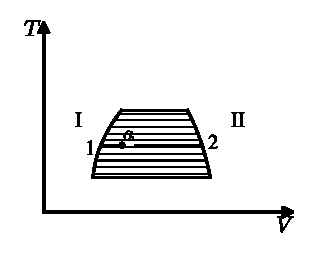
\includegraphics[width=6.5cm]{fig12.pdf}\\[0.3em]{\small 图 12}\end{minipage}\par\nopagebreak

由物质量的均衡很容易直接得出结论：相Ⅰ和相Ⅱ的量反比于线段 $a1$ 和 $a2$ 的长度（所谓杠杆定则）.

类似于两相平衡的条件，同一种物质的三相平衡是由下列各等式来确定的：
\begin{equation}
  P_1=P_2=P_3,\qquad T_1=T_2=T_3,\qquad \mu_1=\mu_2=\mu_3.
\end{equation}
如果用 $P$ 和 $T$ 来重新表示三个相的压强和温度的共同值，那么我们就得到条件
\begin{equation}
  \mu_1(P,T)=\mu_2(P,T)=\mu_3(P,T).
\end{equation}
这是具有两个未知数 $P$ 和 $T$ 的两个方程式；它们的解是一对确定的 $P$ 和 $T$ 值.三个相同时存在的状态（所谓三相点）在 $P$，$T$ 图上用孤立的点来表示，这种点是三相中每两相的平衡曲线的交点（见图13，图中区域Ⅰ，Ⅱ，Ⅲ是三个均匀相的区域）.同一物质的多于三相的平衡显然是不可能的.

在 $T$，$V$ 图上，三相点的邻域具有如图14所示的形式，其中阴影区域是每两个相成对平衡的区域；三相点（温度 $T_{\mathrm{tr}}$）处的平衡态中三相的比体积由点1,2,3的横坐标所确定.

\par\nopagebreak\noindent\begin{minipage}{\linewidth}\centering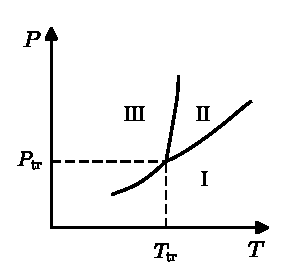
\includegraphics[width=4.8cm]{fig13.pdf}\\[0.3em]{\small 图 13}\end{minipage}\par\nopagebreak

\par\nopagebreak\noindent\begin{minipage}{\linewidth}\centering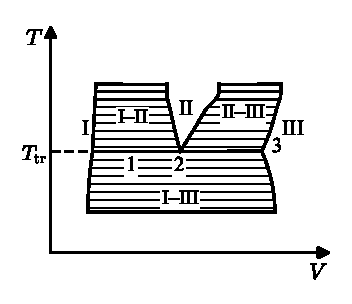
\includegraphics[width=6.5cm]{fig14.pdf}\\[0.3em]{\small 图 14}\end{minipage}\par\nopagebreak

从一个相转变到另一个相，伴随着放出或吸收一定量的热（相变潜热）.按照相平衡条件，这样的相变在恒压和恒温下发生.但是在恒压过程中物体所吸收的热量，等于它的焓变.因此单分子相变潜热 $q$ 是
\begin{equation}
  q=w_2-w_1,
\end{equation}
式中 $w_1$ 和 $w_2$ 是两相的单分子焓.如果从第一相转变到第二相时吸收热量，那么 $q$ 是正的，而相变时放热则 $q$ 为负.

因为（对于由一种物质构成的物体来讲）$\mu$ 是单分子的热力学势，所以可以写成
\begin{equation*}
  \mu=\varepsilon-Ts+Pv
\end{equation*}
（$\varepsilon,s,v$ 是分子的能量、熵和体积）.因此条件 $\mu_1=\mu_2$ 给出：
\begin{equation*}
  (\varepsilon_2-\varepsilon_1)-T(s_2-s_1)+P(v_2-v_1)
  =(w_2-w_1)-T(s_2-s_1)=0,
\end{equation*}
其中 $T$ 和 $P$ 是两个相的温度和压强，由此
\begin{equation}
  q=T(s_2-s_1).
\end{equation}
必须注意：该公式也可以直接取温度恒定从 $q=\int T\,\mathrm{d}s$ 得出.（这个公式在这里适用，因为相变是可逆地进行的——两相在相变过程中保持相互平衡.）

设在图15中的两条曲线表示两相的化学势对温度的函数关系（在给定的压强下）.两条曲线的交点确定两相能够彼此处于平衡的温度 $T_0$（在给定的压强下）.在所有其余的温度下，能够存在的只能是这一相或另一相.很容易看出：在低于 $T_0$ 的温度下，存在的是第一相，亦即稳定的是第一相；而在高于 $T_0$ 的温度下，是第二相，这个结论是从这一点得出的：稳定的状态是 $\mu$ 较小的那种状态（因为在给定 $P$ 和 $T$ 的条件下，热力学势趋向于极小值）.另一方面，在两条曲线的交点上，偏导数 $\dfrac{\partial\mu_1}{\partial T}$ 的值大于 $\dfrac{\partial\mu_2}{\partial T}$ 的值，也就是说，第一相的熵 $s_1=-\dfrac{\partial\mu_1}{\partial T}$ 小于第二相的熵 $s_2=-\dfrac{\partial\mu_2}{\partial T}$，因此，相变潜热 $q=T(s_2-s_1)$ 是正的.因此，我们得出结论：如果当温度升高时物体从一个相转变成另一个相，那么这时就吸收热量.这个结果也可以从勒夏特列原理得出.

\par\nopagebreak\noindent\begin{minipage}{\linewidth}\centering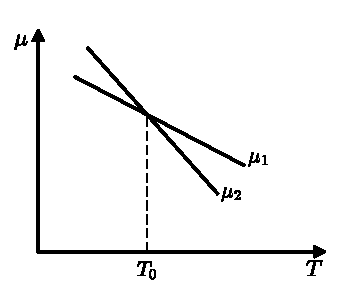
\includegraphics[width=5.5cm]{fig15.pdf}\\[0.3em]{\small 图 15}\end{minipage}\par\nopagebreak

\begin{xiti}

\noindent{\heiti 习题1}\quad 试求出在固体上的饱和蒸气压的温度依赖关系.（把饱和蒸气考虑为理想气体；固体和气体都具有恒定的比热.）

解：蒸气的化学势由公式(43.3)所确定，而固体的化学势由公式(65.6)所确定.（由于饱和蒸气压相对地讲很小，对于固体可以忽略掉 $PV$ 这个量而认为 $\Phi$ 等于 $F$.）令两式相等，我们就求出：
\begin{equation*}
  P=\text{常数}\cdot T^{(c_{p2}-c_1)}\mathrm{e}^{(\varepsilon_{01}-\varepsilon_{02})/T},
\end{equation*}
其中角标1指固体，角标2指蒸气.

在同样的近似下，可以认为固体的焓等于它的能量；相变潜热（升华热）$q=w_2-w_1$ 等于
\begin{equation*}
  q=(c_{p2}-c_1)T+(\varepsilon_{02}-\varepsilon_{01}).
\end{equation*}
特别是，在 $T=0$ 时的相变潜热是 $q_0=\varepsilon_{02}-\varepsilon_{01}$，以致可以写成
\begin{equation*}
  P=\text{常数}\cdot T^{(c_{p2}-c_1)}\mathrm{e}^{-q_0/T}.
\end{equation*}

\noindent{\heiti 习题2}\quad 试求凝聚体蒸发到真空中的蒸发率.

解：蒸发到真空中去的蒸发率由单位时间内离开物体的单位表面积的粒子数来确定.我们考虑同它自己的饱和蒸气处于平衡的物体.于是离开物体表面的粒子数，等于在同样时间内落到这个表面上并“附着”到它上面的粒子数，也就是说等于
\begin{equation*}
  \frac{P_0}{\sqrt{2\pi mT}}(1-R),
\end{equation*}
式中 $P_0=P_0(T)$ 是饱和蒸气压，$R$ 是气体同物体表面发生碰撞时气体粒子的平均“反射系数”（参看(39.2)）.如果 $P_0$ 不太大，则离开物体表面的粒子数与它周围的空间中是否有蒸气存在无关，因此上面所写的式子就确定了我们所求的蒸发到真空中的蒸发率.

\end{xiti}

\section{克拉珀龙-克劳修斯方程}

取相平衡条件
\begin{equation*}
  \mu_1(P,T)=\mu_2(P,T),
\end{equation*}
两边对温度求导数.当然，这时必须注意到压强 $P$ 不是独立变量，而是由这个方程式本身所确定的温度函数.因此我们写成：
\begin{equation*}
  \frac{\partial\mu_1}{\partial T}+\frac{\partial\mu_1}{\partial P}\frac{\mathrm{d}P}{\mathrm{d}T}
  =\frac{\partial\mu_2}{\partial T}+\frac{\partial\mu_2}{\partial P}\frac{\mathrm{d}P}{\mathrm{d}T},
\end{equation*}
而且，因为 $(\partial\mu/\partial T)_P=-s$，$(\partial\mu/\partial P)_T=v$（参看(24.12)），我们得到
\begin{equation}
  \frac{\mathrm{d}P}{\mathrm{d}T}=\frac{s_1-s_2}{v_1-v_2},
\end{equation}
式中 $s_1,v_1$ 和 $s_2,v_2$ 是两相的分子熵和分子体积.

在这个公式中，差值 $s_1-s_2$，可以用从一个相转变到另一个相的潜热来表示.把 $q=T(s_2-s_1)$ 代入，我们就求出所谓克拉珀龙-克劳修斯方程
\begin{equation}
  \frac{\mathrm{d}P}{\mathrm{d}T}=\frac{q}{T(v_2-v_1)}.
\end{equation}
这个公式所确定的是：当温度变化时处于平衡的两个相的压强的变化，或是说，压强沿着相平衡曲线随温度的变化.同一公式也可以写成形式
\begin{equation*}
  \frac{\mathrm{d}T}{\mathrm{d}P}=\frac{T(v_2-v_1)}{q},
\end{equation*}
这个公式所确定的是：当压强变化时两相相变温度（如冰点和沸点）的变化.因为气体的分子体积总是大于液体的分子体积，而当液体转变成气体时吸收热量，因此当压强增加时沸点的温度总是升高$\left(\dfrac{\mathrm{d}T}{\mathrm{d}P}>0\right)$.当压强增加时冰点的温度是升高还是降低，视溶化时体积增加或是减小而定\footnote{例外的情况是氦的同位素 ${}^3\mathrm{He}$，在一定的温度区间内溶解热是负的.}.

公式(82.2)的所有这些结论与勒夏特列原理完全一致.例如，我们来考虑液体同它自己的饱和蒸气处于平衡的情形.如果增加压强，则沸点的温度应当升高；由于这个缘故，一部分蒸气转变成液体，这又转而引起压强的降低；也就是说，系统对于使它离开平衡状态的外作用就好像起着反作用一样.

我们来考虑公式(82.2)的一个特例，即讨论固体或液体同它的蒸气的平衡的情形.这时公式(82.2)所确定的是饱和蒸气压随温度的变化.

气体的体积通常比包含同样数目粒子的凝聚体的体积大得多.因此在(82.2)中，相对于体积 $v_2$ 可略去体积 $v_1$（我们把气体作为第二相），也就是说，取 $\dfrac{\mathrm{d}P}{\mathrm{d}T}=\dfrac{q}{Tv_2}$.把蒸气考虑为理想气体，我们可以按照克拉珀龙公式 $v_2=\dfrac{T}{P}$，把它的体积用压强和温度来表示；于是我们得到：
\begin{equation*}
  \frac{\mathrm{d}P}{\mathrm{d}T}=\frac{qP}{T^2},
\end{equation*}
即
\begin{equation}
  \frac{\mathrm{d}\ln P}{\mathrm{d}T}=\frac{q}{T^2}.
\end{equation}
我们看到：在相变潜热可以认为是常数的温度区，饱和蒸气压按照指数规律$\left(\propto\exp(-q/T)\right)$随温度而变化.

\begin{xiti}

\noindent{\heiti 习题1}\quad 试求出沿着液体及其饱和蒸气的平衡曲线变化时（即在液体一直同它的饱和蒸气处于平衡的过程中）的蒸气比热.蒸气可以认为是理想气体.

解：所求的比热 $h$ 等于
\begin{equation*}
  h=T\frac{\mathrm{d}s}{\mathrm{d}T},
\end{equation*}
式中 $\dfrac{\mathrm{d}s}{\mathrm{d}T}$ 是沿着相平衡曲线取的导数，即
\begin{equation*}
  h=T\frac{\mathrm{d}s}{\mathrm{d}T}
  =T\left(\frac{\partial s}{\partial T}\right)_P
  +T\left(\frac{\partial s}{\partial P}\right)_T\frac{\mathrm{d}P}{\mathrm{d}T}
  =c_p-T\left(\frac{\partial v}{\partial T}\right)_P\frac{\mathrm{d}P}{\mathrm{d}T}.
\end{equation*}
把(82.3)式的 $\dfrac{\mathrm{d}P}{\mathrm{d}T}$ 和 $v=\dfrac{T}{P}$ 代入上式，我们求出：
\begin{equation*}
  h=c_p-\frac{q}{T}.
\end{equation*}
在低温下，$h$ 是负的，也就是说，如果可以取走热量，以使得蒸气一直同液体处于平衡，那么它的温度可以升高.

\noindent{\heiti 习题2}\quad 试求出在蒸气一直同液体处于平衡的过程中（即沿着液体及其蒸气的平衡曲线）蒸气体积随温度的变化.

解：导数 $\dfrac{\mathrm{d}v}{\mathrm{d}T}$ 必须沿着相平衡曲线来确定：
\begin{equation*}
  \frac{\mathrm{d}v}{\mathrm{d}T}
  =\left(\frac{\partial v}{\partial T}\right)_P
  +\left(\frac{\partial v}{\partial P}\right)_T\frac{\mathrm{d}P}{\mathrm{d}T}.
\end{equation*}
把(82.3)和体积 $v=\dfrac{T}{P}$ 代入上式，我们求出：
\begin{equation*}
  \frac{\mathrm{d}v}{\mathrm{d}T}=\frac{1}{P}\left(1-\frac{q}{T}\right).
\end{equation*}
在低温下 $\dfrac{\mathrm{d}v}{\mathrm{d}T}<0$，也就是说，在所考虑的过程中，蒸气的体积随温度的增加而减小.

\end{xiti}

\section{临界点}

相平衡曲线（在 $PT$ 平面上）可能在某一点终止（图16）；这样的点称为临界点，而与它相对应的温度和压强称为临界温度和临界压强.在高于 $T_{\mathrm{c}}$ 的温度和大于 $P_{\mathrm{c}}$ 的压强下，不存在不同的相，而物体总是均匀的.可以说：在临界点，两相之间的差别完全消失.临界点的概念是由 Д.~И.~门捷列夫首先提出的(1860).

在以 $T,V$ 为坐标的有临界点存在的平衡图看上去就像图17所描绘的样子.当温度趋近于它的临界值时，彼此处于平衡的两相的比体积也逐渐接近，而在临界点（图17中的 $K$）完全等同.以 $P,V$ 为坐标的平衡图具有类似的形式.

\par\nopagebreak\noindent\begin{minipage}{\linewidth}\centering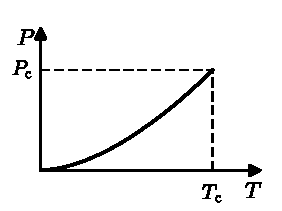
\includegraphics[width=4.5cm]{fig16.pdf}\\[0.3em]{\small 图 16}\end{minipage}\par\nopagebreak

\par\nopagebreak\noindent\begin{minipage}{\linewidth}\centering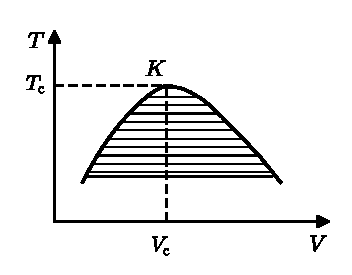
\includegraphics[width=6cm]{fig17.pdf}\\[0.3em]{\small 图 17}\end{minipage}\par\nopagebreak

当存在着临界点时，一种物质的任何两态之间可以发生连续的相变，在这种相变过程中，任何时刻物质都不会分离成两相——要做到这一点，只需要沿着任何一条绕过临界点而与相平衡曲线从不相交的曲线来改变物质的状态.在这种意义下，当有临界点存在时，关于不同相的概念本身有随意性，不可能在所有情况下指出：什么样的状态是这一相，什么样的状态是另一相.严格地讲，只有当两相彼此接触而同时存在时，亦即只有在相平衡曲线的诸点上，才可以说两相.

显然，只有当两相之间仅具有纯粹定量的差别时，对于这样的两相才可能有临界点存在.液体和气体就是这样，它们的区别只在于分子间相互作用的大小程度不同.

至于像物质的液体和固体（晶体）或各种晶态这样的相，则彼此间有质的差别，因为它们各自的内部对称性不同.显然，对于任何对称性质（对称元素）我们只能说它存在，或者它不存在；它只可能即刻、突发地出现或消失，而不可能逐渐地出现或消失.在每一种这样的状态，物体或者具有这一种对称，或者具有另一种对称，因而总是可以指出物体在两相中间属于哪一相.因而对于这样的相，临界点是不可能存在的，而相平衡曲线必然或者延伸到无限远，或者同其它各相的平衡曲线相交而终止.

通常的相变点并不是物质热力学量的数学奇点.实际上，每一相也可以在相变点的另一侧存在（虽然是亚稳的）；热力学不等式在这一点并未破坏.在相变点，两相的化学势只是彼此相等而已 $\mu_1(P,T)=\mu_2(P,T)$；对于函数 $\mu_1(P,T)$ 和 $\mu_2(P,T)$ 的任一个来讲，这一点毫无特殊之处\footnote{然而，必须指出，这种说法是有条件的，因为在亚稳区 $\mu(P,T)$ 的概念有某种不确定性. 亚稳态是不完全平衡，具有某种弛豫时间（在这里相应于新相成核过程，参看§162）. 所以，这种状态下热力学函数只有在不考虑这些过程时才能定义，而且不能把它们看成是（对应于物质完全平衡态的）稳定区函数的解析开拓.}.

我们在 $PV$ 平面上画一条液体和气体的等温线，也就是当均匀物体等温膨胀时 $P$ 对 $V$ 的关系的曲线（图18上的 $abc$ 和 $def$）.根据热力学不等式 $\left(\dfrac{\partial P}{\partial V}\right)_T<0$，$P$ 是 $V$ 的减函数.等温线的这样的斜率必然一直保持到它们同液体和气体的平衡曲线的交点（点 $b$ 和点 $e$）以外的一段延伸线上；等温线的片段 $bc$ 和 $ed$ 各对应于亚稳的过热液体和过冷蒸气，在这两段上，热力学不等式仍旧保持.

\par\nopagebreak\noindent\begin{minipage}{\linewidth}\centering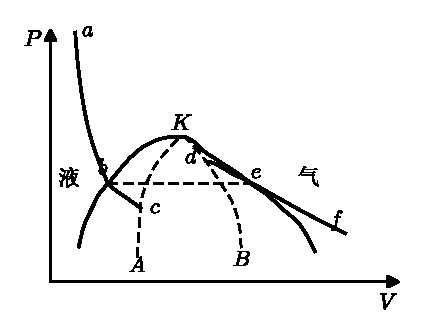
\includegraphics[width=8cm]{fig18.pdf}\\[0.3em]{\small 图 18}\end{minipage}\par\nopagebreak

（当然，在点 $b$ 和点 $e$ 之间的完全平衡的状态等温变化，对应于水平线段 $be$，那里发生两相分离.）如果考虑到点 $b$ 和点 $e$ 具有同样的纵坐标 $P$，那么，显然等温线的两部分不可能以连续的方式彼此过渡，它们之间必然有间断.等温线在点 $c$ 和点 $d$ 终止，在这两点热力学不等式被破坏，即
\begin{equation}
  \left(\frac{\partial P}{\partial V}\right)_T=0.
\end{equation}
把液体和气体等温线的终点轨迹标绘出来，我们就得到一条曲线（图18上的 $AKB$），在这条曲线上，热力学不等式（对于均匀物体来讲）破坏；它限定了一个区域，在任何条件下物体在其中都不可能以均匀的状态存在.在这条曲线和相平衡曲线之间的区域是过热液体和过冷蒸气可能存在的区域\footnote{等温线上相应于过热液体的片段（图 18 上的 $bc$）可以部分地位于横轴之下. 换句话说，过热液体可以具有负压强；这样的液体作用到它的制约表面上的力指向液体体积内部. 由此可见，压强未必为正，在自然界中物体可以有压强值为负的（虽然只是亚稳的）状态.（关于这一点，在§12中已经讲过.）}.显然，在临界点，两条曲线应当彼此相触.至于正好在曲线 $AKB$ 上的各点中，只有临界点 $K$ 对应于均匀物体实际存在的状态；它是这条曲线同稳定均匀状态区接触的唯一一点.

值得指出，在临界点处的条件(83.1)也可以由下面的简单考虑得到.在临界点附近，液体和蒸气的比体积彼此接近.用 $V$ 和 $V+\delta V$ 来表示它们，我们就可以把两相压强相等的条件写成形式
\begin{equation}
  P(V,T)=P(V+\delta V,T).
\end{equation}
把等式右边按 $\delta V$ 的幂次展开，再除以很小而有限的量 $\delta V$，我们就求出：
\begin{equation}
  \left(\frac{\partial P}{\partial V}\right)_T
  +\frac{\delta V}{2}\left(\frac{\partial^2P}{\partial V^2}\right)_T+\cdots=0.
\end{equation}
由此看出：当 $\delta V$ 趋向于0时，亦即在临界点处，$\left(\dfrac{\partial P}{\partial V}\right)_T$ 在任何情形下都应当变成0.

与普通的相平衡点相反，临界点是物质热力学函数的数学奇点（限制物体均匀状态存在区域的整条曲线 $AKB$ 也是这样）.物质在临界点附近的奇异性与行为将在§153中研究.

\section{对应态定律}

范德瓦尔斯的内插物态方程
\begin{equation}
  P=\frac{NT}{V-Nb}-\frac{N^2a}{V^2},
\end{equation}
同液体和蒸气之间的相变的上述性质定性地符合.

由这个方程所确定的等温线如图19所示.通过临界点 $K$ 上方的一些曲线表示 $T>T_{\mathrm{c}}$ 时的单调减函数 $P(V)$.穿越临界点的等温线在那里有拐点.在温度 $T<T_{\mathrm{c}}$ 时，每条等温线都有极小值和极大值，二者其间为 $\left(\dfrac{\partial P}{\partial V}\right)_T>0$ 的一段；这些段（在图19中用虚线表示）并不与自然界中实际存在的任何物质均匀态对应.

\par\nopagebreak\noindent\begin{minipage}{\linewidth}\centering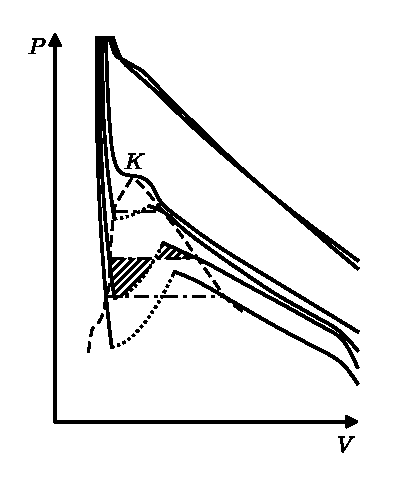
\includegraphics[width=7cm]{fig19.pdf}\\[0.3em]{\small 图 19}\end{minipage}\par\nopagebreak

正如上节已经阐明的，与等温线相交的水平线段相应于液体到气体的平衡相变.该线段应该在的水平位置取决于相平衡条件 $\mu_1=\mu_2$，我们把它写成
\begin{equation*}
  \int_1^2\mathrm{d}\mu=0,
\end{equation*}
式中积分沿着从一个相的状态过渡到另一个相的状态的路径求.等温线上有 $\mathrm{d}\mu=v\,\mathrm{d}P$，因此沿等温线求积分
\begin{equation}
  \int_1^2V\,\mathrm{d}P=0.
\end{equation}
在几何上，这个条件表示图19中对一条等温线画的阴影面积相等（麦克斯韦法则）.

临界温度、压强和体积可以用范德瓦尔斯方程中所含的参量 $a$ 和 $b$ 来表示.为此，对表达式(84.1)求微商并且写出确定等温线拐点的方程
\begin{equation*}
  \left(\frac{\partial P}{\partial V}\right)_T=0,\qquad
  \left(\frac{\partial^2P}{\partial V^2}\right)_T=0,
\end{equation*}
它们与(84.1)式一起给出
\begin{equation}
  T_{\mathrm{c}}=\frac{8}{27}\frac{a}{b},\qquad
  V_{\mathrm{c}}=3Nb,\qquad
  P_{\mathrm{c}}=\frac{1}{27}\frac{a}{b^2}.
\end{equation}
现在我们引入如下定义的温度、压强和体积
\begin{equation}
  T'=\frac{T}{T_{\mathrm{c}}},\qquad
  P'=\frac{P}{P_{\mathrm{c}}},\qquad
  V'=\frac{V}{V_{\mathrm{c}}}
\end{equation}
采用这些量，范德瓦尔斯方程取如下形式
\begin{equation}
  \left(P'+\frac{3}{V'^2}\right)(3V'-1)=8T'.
\end{equation}
这个方程只含有 $V',P'$ 和 $T'$，而并不含任何表征该物质的量.因此方程(84.5)是范德瓦尔斯方程适用的所有物体的物态方程.两个物体具有同样的 $T',P',V'$ 时，它们的状态称为对应态（显然，所有物体的临界状态都是对应态）.由(84.5)得出结论：如果两个物体在 $T',P',V'$ 这三个量中有两个相等，那么第三个也相等，也就是说，它们处于对应态（对应态定律）.

由方程式(84.5)所确定的“约化”等温线 $P'=P'(V')$ 对于所有的物质都是相同的.因而，确定液体到气体相变点的直线段也有一样的位置.因此可以得出结论：在同样的约化温度下，所有的物质应当具有同样的如下各量：1）约化饱和蒸气压，2）饱和蒸气约化比体积，3）与饱和蒸气处于平衡的液体的约化比体积.

对应态定律也可以应用于液态到气态的相变潜热上.这时“约化蒸发热”应当由一个无量纲量即 $\dfrac{q}{T_{\mathrm{c}}}$ 充当.因此可以写成\footnote{温度显著低于临界点时，比值 $\dfrac{q}{T_{\mathrm{c}}}$ 约等于 10（$q$ 为分子蒸发热）.}：
\begin{equation}
  \frac{q}{T_{\mathrm{c}}}=f\left(\frac{T}{T_{\mathrm{c}}}\right).
\end{equation}
最后我们指出，对应态定律并非专指范德瓦尔斯方程.当仅含有两个参量的任意物态方程转为约化量时，表征具体物质的参量消失.对应态定律，作为不局限于物态方程某种具体形式的一般结论，本身比范德瓦尔斯方程多少更精确些.但是，一般说来其适用性仍十分有限.
